\chapter{Herramientas y tecnologías}

%%%%%%%%%%%%%%%%%%%%%%%%%%%%%%%%%%% Chisel %%%%%%%%%%%%%%%%%%%%%%%%%%%%%%%%%%%%

\section{Chisel}

Chisel es un lenguaje de descripción de hardware de alto nivel gestado en el año 2012 en el seno del Departamento de Ingeniería Eléctrica y Ciencias de la Computación (abrev. EECS) de la Universidad de California, en Berkeley, y surgió como parte de un proyecto de investigación cuyo objetivo final era la implementación de una interfaz de lenguaje con la que elevar el nivel de abstracción ofrecido por HDL's convencionales como son VHDL o Verilog, ofreciendo la posibilidad de traducir los desarrollos elaborados, en entidades descritas en estos mismos lenguajes de bajo nivel, con objeto de correr procesos de síntesis o emulación que permitiesen evaluar su funcionamiento \cite{chiselEECS}.

El hecho de que se trate de un HDL de alto nivel tiene un impacto directo y positivo sobre la celeridad en los procesos de desarrollo y prueba del hardware, permitiendo elaborar y probar diseños de una manera ágil sin perder las características de eficiencia y robustez que proporcionan lenguajes de más bajo nivel.

Es un lenguaje de propósito específico construido sobre Scala, un lenguaje de propósito general orientado a objetos, siendo esta la principal propiedad que permite a Chisel mostrar al usuario una interfaz de diseño de hardware de tan alto nivel y, por ende, amigable tanto para el desarrollador novel como para usuarios más avanzados, y es que resulta muy práctico el poder modelar un circuito lógico como un conjunto de clases relacionadas entre sí, cada una de ellas definiendo su funcionamiento interno particular, y constituyendo esas relaciones, conexiones entre los diferentes módulos de los que se componga el diseño global.

\subsection{Desarrollo en Chisel}

La unidad fundamental de diseño de hardware en Chisel son los módulos, que encapsulan la disposición interna y el comportamiento de un circuito lógico. Esta disposición interna pueden componerla otros módulos, cables internos o cables de entrada/salida, cuyos valores serán empleados en la evaluación de las expresiones lógicas que definan el comportamiento del módulo, y que pueden describirse por medio de operadores aritmético-lógicos convencionales, o bien, por medio de los tipos de datos y componentes definidos en las librerías de Chisel, tales como multiplexores, decodificadores o incluso memorias.

A continuación, en la Figura 3.1, se proporciona un código sencillo con el que se describe un multiplexor de 4 entradas de 32 bits cada una. Nótese que los módulos se definen como clases que extienden la clase \textit{Module}, lo cual hace mandatorio que se cuente con, al menos, una interfaz encapsulada en el método \textit{IO}, por medio del cual se definirá esa interfaz como un elemento de entrada/salida. En el caso del código mostrado en la Figura 3.1 las interfaces de entrada/salida se encuentran definidas en las líneas 7 a 14 como parte de una instancia de la clase \textit{Budle}, que es un constructo que permite en Chisel crear nuevos tipos de datos al estilo de los \textit{struct} en el lenguaje C.

\begin{figure}
\begin{lstlisting}[style=scalaStyle]{}
package mux4

import chisel3._
import chisel3.util._

class Mux4 extends Module {
  val io = IO(new Bundle{
    val i1  = Input(UInt(32.W))
    val i2  = Input(UInt(32.W))
    val i3  = Input(UInt(32.W))
    val i4  = Input(UInt(32.W))
    val sel = Input(UInt(2.W))

    val o   = Output(UInt(32.W))
  })

  io.o := MuxLookup(io.sel, io.i1)(
    Seq(
      0.U -> io.i1,
      1.U -> io.i2,
      2.U -> io.i3,
      3.U -> io.i4,
    ))
}
\end{lstlisting}
\caption{Definición de un multiplexor sencillo en Chisel}
\end{figure}

\subsection{Pruebas en Chisel}

Como se comentaba al comienzo de esta sección sobre Chisel, una de sus características más reseñables es la agilidad con la que puede probarse el comportamiento de los módulos, y ello es gracias a los tests, los cuales son definiciones de clases que implementan uno de los \textit{traits} de Chisel en los que se definen a su vez los procedimientos que permiten evaluar el funcionamiento de los módulos. Estos \textit{traits} son interfaces que definen una serie funciones básicas con las que comprobar y alterar el estado de las señales dentro de los módulos.

Estas interfaces han ido cambiando conforme evolucionaba el propio HDL y, a pesar de no ser la forma de prueba mantenida en las últimas versiones de Chisel, que sería \textit{ChiselSim}, se ha decidido utilizar \textit{ChiselScalatestTester} como interfaz de pruebas, puesto que desde el punto de vista de la implementación no se encuentran grandes diferencias entre ellas, además de que es la forma de prueba utilizada en el proyecto base.

Las interfaces de prueba de Chisel definen cuatro funciones básicas con las que evaluar el comportamiento de un módulo: \textit{peek}, \textit{poke},  \textit{expect} y \textit{step}. Estas funciones se invocan sobre las diferentes señales de las cuales se componga el módulo y permiten realizar las siguientes acciones:

\begin{itemize}
  \item \textbf{\textit{peek}}: lectura del valor de una señal en el instante de invocación de la función.
  \vspace{-0.2cm}
  \item \textbf{\textit{poke}}: cambio en el valor de la señal.
  \vspace{-0.2cm}
  \item \textbf{\textit{expect}}: evaluación de un valor determinado en la señal, esto es, probar si el valor de la señal en el instante de invocación de la función es el esperado.
  \vspace{-0.2cm}
  \item \textbf{\textit{step}}: se invoca sobre una señal de reloj y permite avanzarlo un ciclo.
\end{itemize}

En la Figura 3.2 se muestra un ejemplo de test que evalúa el comportamiento del módulo definido en el código de la Figura 3.1.

\begin{figure}
\begin{lstlisting}[style=scalaStyle]{}
package mux4

import chisel3._
import chiseltest._
import org.scalatest.flatspec.AnyFlatSpec
import mux4.Mux4

class Mux4Test extends AnyFlatSpec with ChiselScalatestTester {
  behavior.of("Mux4")
  it should "generate the right output given any valid selector value as input" in {
    test(new Mux4) { c =>
      c.io.i1.poke(1.U)
      c.io.i2.poke(2.U)
      c.io.i3.poke(3.U)
      c.io.i4.poke(4.U)
      var x = 0
      for (x <- 0 to 3) {
        c.io.sel.poke(x.U)
        c.io.o.expect(x + 1)
      }
    }
  }
}
\end{lstlisting}
\caption{Implementación de un test para el multiplexor de 4 entradas}
\end{figure}

%%%%%%%%%%%%%%%%%%%%%%%%%%%%%%%%%%%%% SBT %%%%%%%%%%%%%%%%%%%%%%%%%%%%%%%%%%%%%

\section{SBT}

SBT es una herramienta de construcción de software semejante a Maven o Gradle, y es la más utilizada por los desarrolladores en lenguaje Scala\cite{scalaSurvey}.

Su uso es por medio de una interfaz de línea de comandos, proporcionando una consola interactiva desde la que pueden realizarse todo tipo de tareas administrativas sobre los proyectos, tales como lanzar pruebas, ejecutar un programa principal, compilar ficheros de código fuente de manera individual o construir el proyecto, requirendo esto último la creación de un fichero de configuración \textit{build.sbt} dentro del directorio del proyecto.

Escrito también en el lenguaje Scala, en él se definirán las propiedades del proyecto, como puedan ser su nombre y versión, la versión de Scala empleada en la implementación o las librerías de las que depende, siendo estas dos últimas propiedades imprescibdibles de cara al proceso de compilación.

En la Figura 3.3 se proporcionan ejemplos de uso de la consola de SBT, primero, invocando el proceso de elaboración del módulo descrito en la sección 3.1 mediante el comando \textit{compile} y, acto seguido, lanzando el test desarrollado, previa elaboración de este.

\vspace{+0.3cm}
\begin{figure}[h]
  \centering
  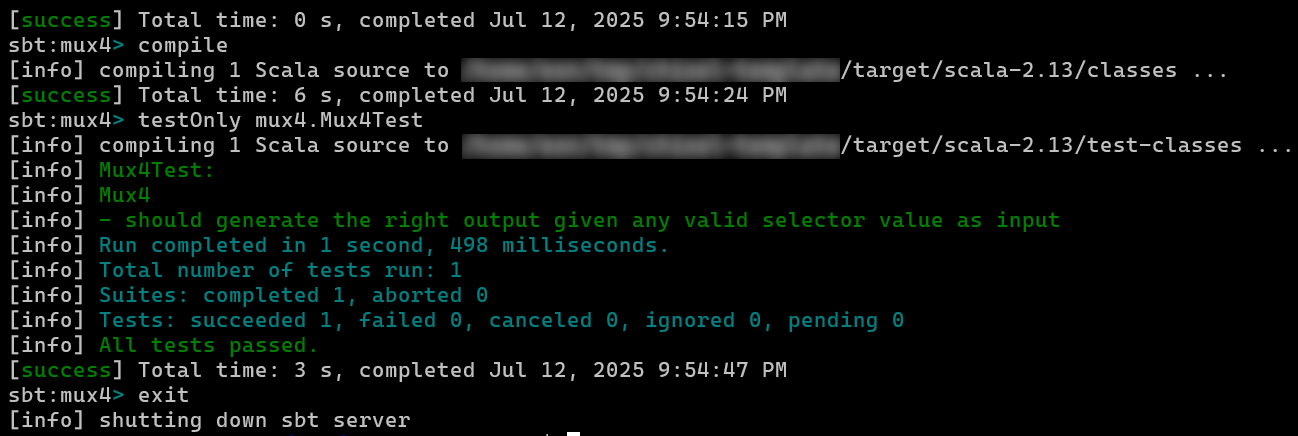
\includegraphics[width=0.8 \linewidth]{res/img/sbt-usage-basic.png}
  \caption{Elaboración y prueba del módulo descrito en la sección 3.1}
\end{figure}

%%%%%%%%%%%%%%%%%%%%%%%%%%%%% RISC-V GNU Toolchain %%%%%%%%%%%%%%%%%%%%%%%%%%%%
\section{RISC-V GNU Toolchain}

Gran parte de las pruebas llevadas a cabo sobre la implementación del núcleo han consistido en la carga, ejecución y depuración de programas desarrollados en lenguaje C, lo cual ha implicado aplicar un proceso de compilación cruzada para obtener binarios que pudieran ejecutar sobre la arquitectura RISC-V.

Este proceso ha sido llevado a cabo por medio de la suite de herramientas de que se compone el toolchain de GNU para RISC-V\cite{riscvtoolchain}, disponible en sistemas Linux basados en Debian por medio del gestor de paquetes \textit{apt} (paquete \textit{gcc-riscv64-unknown-elf}).

%%%%%%%%%%%%%%%%%%%%%%%%%%%%%%%%%%% GTKWave %%%%%%%%%%%%%%%%%%%%%%%%%%%%%%%%%%%
\section{GTKWave}

La depuración de componentes arquitecturales individuales tales como la ALU o el banco de registros, o incluso fases completas dentro del pipeline, es una tarea que puede acometerse de manera ágil por medio de tests, estableciendo primeramente los casos de prueba a implementar, y verificando que los cambios en las señales bajo supervisión son los esperados para el conjunto de entradas definido en cada caso de prueba. No obstante, este proceso de depuración del pipeline se torna más complejo cuando se desea verificar el comportamiento global de la arquitectura mediante la ejecución de un programa, lo cual requiere la implementación de tests que verifiquen el estado de un número mucho mayor de señales a cada ciclo, incrementando notablemente la complejidad de los tests desarrollados y del proceso de depuración.

Aún siendo esta una tarea ciertamente abordable, se optó por explorar alternativas que permitiesen depurar el estado de la arquitectura de una manera más rápida y visual, y se consideró que la herramienta GTKWave cumpliría perfectamente con este propósito.

GTKWave es una herramienta de análisis empleada en la depuración de trazas generadas en los procesos de simulación de modelos elaborados con Verilog o VHDL. Estas trazas, generadas con la ejecución de los tests de Chisel, se almacenan en ficheros con un formato definido originalmente en el estándard IEEE 1364-1995\cite{IEEE1364} y constituyen una descripción de todos los cambios experimentados por las señales de los módulos durante la ejecución de las simulaciones.

La herramienta permite explorar esos cambios de una manera visual por medio de una interfaz gráfica en la que puede explorarse el histórico de cambios de la totalidad de las señales que conformen cada módulo, tal y como se muestra en la Figura 3.4, donde se presenta una captura de pantalla de la interfaz gráfica de GTKWave, mostrando una visualización de la traza generada tras la ejecución de un test semejante al mostrado en la Figura 3.2, adaptado para que los cambios en las señales se reflejen en la traza, algo que no se conseguía con la implementación original.

\vspace{+0.5cm}
\begin{figure}[h]
  \centering
  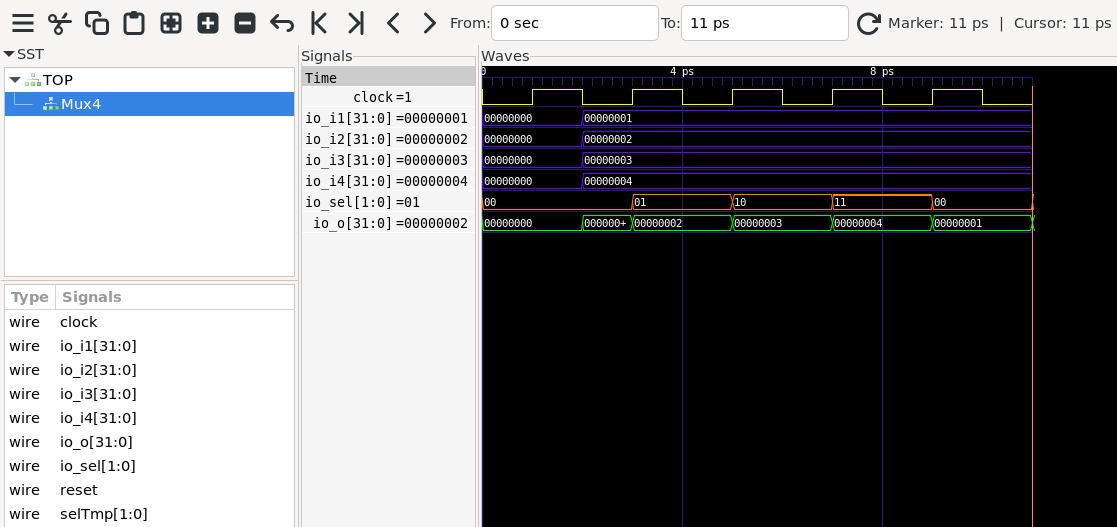
\includegraphics[width=0.8\linewidth]{res/img/test_mux4_gtkwave.png}
  \caption{Visualización de la traza generada tras la simulación del test}
\end{figure}

%%%%%%%%%%%%%%%%%%%%%%%%%%%% Artix A7 y AMD Vivado %%%%%%%%%%%%%%%%%%%%%%%%%%%%
\section{FPGA Artix A7 y AMD Vivado Design Suite}

AMD Vivado es un software de diseño hardware para SoC\footnote{System-on-Chip: circuitos integrados que incorporan todos o la gran mayoría de los componentes que constituyen un computador} y FPGAs desarrollado y mantenido por la empresa AMD que es, además, el fabricante de la placa de desarrollo Artix A7 empleada en las pruebas llevadas a cabo como parte del proceso de verificación final de la arquitectura diseñada.

La placa alberga el FPGA AMD (anteriormente Xilinx) Artix-100T, con 101440 celdas lógicas\cite{arty}, superficie más que suficiente para albergar el núcleo segmentado.

%%%%%%%%%%%%%%%%%%%%%%%%%%%%%% Logisim Evolution %%%%%%%%%%%%%%%%%%%%%%%%%%%%%%
\section{Logisim Evolution}

Se trata de un software CAD de código abierto utilizado para el diseño y simulación de circuitos lógicos, y fue la herramienta empleada para la creación de los diagramas de la arquitectura que se mostrarán en capítulos posteriores de esta memoria.

%%%%%%%%%%%%%%%%%%%%%%%%%%%%%%%%%%%%% Git %%%%%%%%%%%%%%%%%%%%%%%%%%%%%%%%%%%%%
\section{Git}

Git fue concebido originalmente por Linus Torvalds como una alternativa de código abierto a BitKeeper, el software de control de versiones propietario empleado en el desarrollo del kernel de Linux entre los años 2002 y 2005\cite{githistory}, y es actualmente el software de control de versiones más utilizado por los desarrolladores, según los datos reflejados en el \textit{Stack Overflow Annual Developer Survey} del año 2022\cite{stackoverflow}